\section{Metodología}

\textbf{Metodología en V}\\
Para el desarrollo del sistema se tomará como base la metodología en V. 
Elegimos esta metodología debido a que nuestro sistema se compone tanto de software como de hardware, por lo que las etapas que la conforman se adecúan perfectamente para el desarrollo de esta clase de sistemas como a continuación se explicará. 
La metodología indica que se debe de partir de la especificación de requisitos tanto para software como para hardware, en esta etapa se definen los requerimientos funcionales, técnicos y no funcionales, trazando un plan para el diseño del sistema mediante casos de uso, comprendiendo las limitaciones, identificando el impacto del mismo y previendo posibles cambios. En la siguiente etapa se realiza un diseño de alto nivel con base en la información recogida sobre requisitos y análisis, permitiendo obtener un diseño y una visión general del sistema. 
A continuación, se realiza un diseño en detalle, donde veremos al sistema de manera modular, en nuestro caso contamos con un total de tres módulos, teniendo así la ventaja de rediseñar un módulo en específico, hacer cambios de manera efectiva y reducir costos por modificaciones futuras. Posteriormente, el diseño es implementado con el lenguaje de programación elegido para cada módulo, obteniendo programas ejecutables capaces de ofrecer la funcionalidad esperada. A su vez, cada módulo va a ser sometido a pruebas para validar el análisis y diseño previamente realizado \citep{Metodologia1}.
\\
Las pruebas de cada nivel son descritas a continuación:

\begin{itemize}

    \item Pruebas unitarias/modulares: Estas pruebas comprueban que todas las funcionalidades especificadas en el diseño del componente sean correctas y cubiertas, estas pruebas son realizadas por el desarrollador del componente.
    
    \item Pruebas de integración/interfaz: Una vez que los módulos han sido probados de manera unitaria, se procede a probar su funcionalidad de manera conjunta, estas pruebas están enfocadas a resolver los siguientes supuestos:
    
    \begin{itemize}
        \item Que espera un componente de otro componente, en término de servicios.
        \item Como es que estos servicios serán solicitados.
        \item Como es que estos servicios serán entregados.
        \item El manejo de errores por condiciones inesperadas.
    \end{itemize}
    
    Las pruebas deben corroborar el correcto funcionamiento de todas las interfaces entre componentes, al tener todos los componentes y sus interfaces terminados, tendremos como resultado el sistema completo, estas pruebas pueden ser realizadas por el desarrollador del componente.
    
    \item Pruebas del sistema: Una vez el sistema ha sido construido, debe ser probado contra las especificaciones del sistema para comprobar que cubra las funcionalidades requeridas.\\
    Esta parte se enfoca en probar el sistema de manera monolítica y debe incluir las pruebas para validar los requerimientos no funcionales.

    \item Pruebas de validación: similar a las pruebas del sistema, pero hay un cambio en el enfoque, ya que éstas comprueban que el sistema cumple con lo requerido, además las pruebas son realizadas por el usuario final del sistema.

\end{itemize}

\\
\begin{figure}[H]
	\centering
	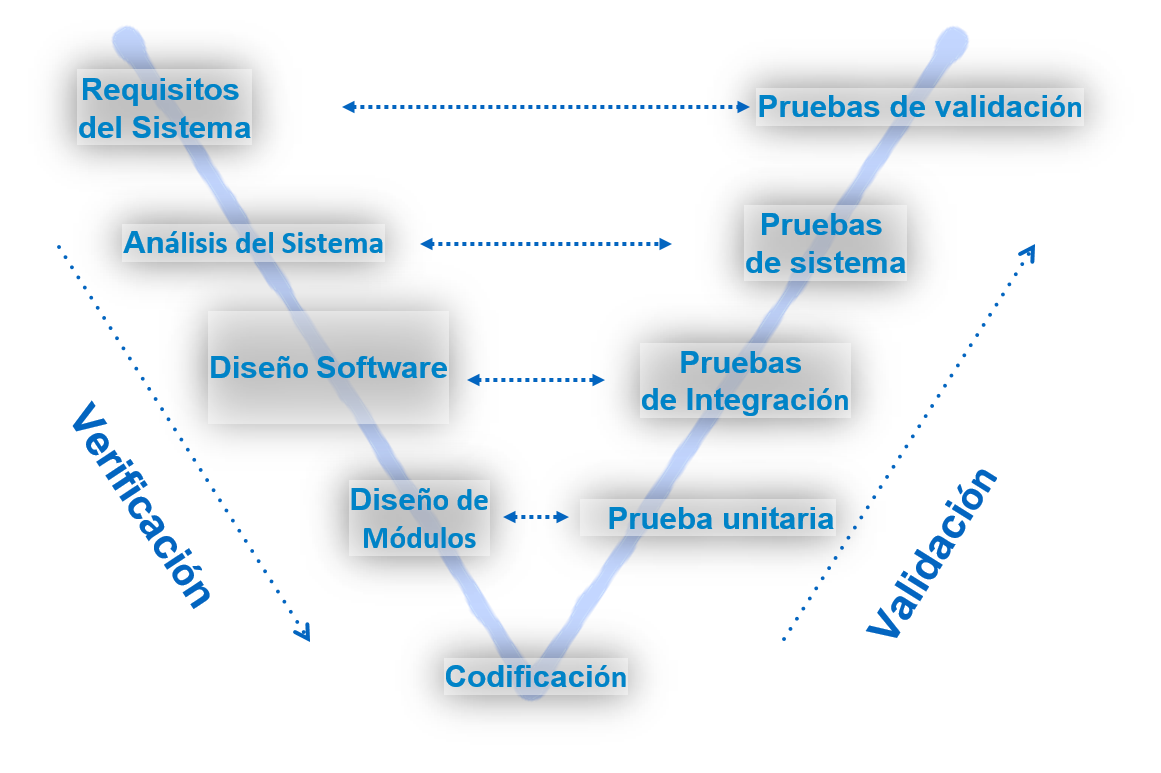
\includegraphics[scale=.4]{Capitulo3/img/vmodel.png}
	\caption{Metodología en V}
	\label{fig:ModeloIncremental}
\end{figure}

